\chapter{Discussão de resultados}

\par Neste capítulo serão apresentados e discutidos os resultados obtidos pela pesquisa e implementação 
do sistema de otimização do processo de fabricação de calças. Tal discussão será realizada em forma de
casos de teste, buscando demonstrar o comportamento do algoritmo genético de diferentes formas.

\par Desde o princípio, quando começou-se a discutir sobre o tema do 
trabalho de conclusão de curso, teve-se a ideia de desenvolver algo relacionado
à inteligência artificial, por ser um assunto de bastante relevância na área de desenvolvimento de software. 
Dentro deste campo então, realizando algumas buscas na internet, foi encontrado
o assunto de algoritmos genéticos.
Coincidentemente foi lecionada no primeiro semestre deste ano a diciplina
sistemas especialistas, a qual o assunto foi abordado o que facilitou bastante o aprendizado.

\par Assim, como sugestão do professor orientador, foi decidido então
desenvolver uma aplicação para otimizar um processo de distribuição de atividades entre
costureiras para um microempresário da cidade de Cachoeira de Minas - MG, do ramo de costura e constatamos 
que um sistema Web seria mais cômodo de ser utilizado por não precisar de
nenhuma instalação por parte do usuário e este poder acessar o programa de
qualquer lugar desde que estivesse conectado à internet.

Neste sentido, foram adotadas como tecnologias para o desenvolvimento em
plataforma Web os \textit{frameworks} JSF e Primefaces. Além disso foi utilizado
um \textit{plug-in} denominado \texttt{JBoss Tool} o qual foi de grande utilidade para gerar as classes 
modelo a partir do banco de dados.

\par Inicialmente foi tomado como base o caso do microempresário citado acima,
todavia logo após iniciarmos o trabalho, o mesmo fez uma reestruturação de processos em sua empresa. 
Desta forma, sua maneira de trabalhar deixou de ser um cenário o qual algoritmos genéticos
pudessem ser aplicados, desta forma, fechou-se um escopo para que o trabalho
pudesse continuar, conforme descrito na seção 3.3.2 do quadro metodológico. Com
o escopo definido, o foco passou a ser na definição da estrutura dos elementos do algoritmo genético.

\par Um dos maiores desafios do trabalho foi a definição da função de avaliação, pois, 
uma vez que existe uma estrutura de nós contendo as atividades e o cálculo do
tempo de cada atividade depende de nós predecessores, a maior parte da função foi 
pensada para ser desenvolvida de forma recursiva o que dificultou o
\textit{debug}.

\par Para a construção do algoritmo genético, foi utilizado uma base desenvolvida pelo professor Artur Barbosa 
durante as aulas de sistemas especialistas, que define uma série de regras a ser
seguida durante o desenvolvimento. Tal base é explicada com mais detalhes no
quadro metodológico e foi de grande ajuda pois, além de definir as
regras, a base já implementava os métodos de seleção e cruzamento, neste sentido
só foi preciso realizar algumas adaptações nestes para que pudessem se
adequar à lógica desenvolvida para resolver o problema.

\par Após ter o escopo definido e a modelagem do algoritmo genético realizada, o
desenvolvimento foi dividido entre os autores e manteve-se as reuniões
periódicas para acertar detalhes do desenvolvimento.

\par Após todas as etapas descritas acima, foi obtido como resultado a aplicação
capaz de distribuir atividades de forma a se obter o menor custo e o menor tempo de produção, 
alcançando assim os objetivos específicos conforme mostra a Figura
~\ref{fig:tela_inicial_da_aplicação}.

\begin{figure}[h!]
	\centerline{
\includegraphics[scale=0.3]{./imagens/tela_inicial.png}}
	\caption[Tela inicial da aplicação]
	{Tela inicial da aplicação \textbf{Fonte:} Desenvolvido pelos autores}
	\label{fig:tela_inicial_da_aplicação}
\end{figure}


\par Com a aplicação finalizada, foram realizados então casos de testes a fim de colocar em prova a eficiência da ferramenta para se 
buscar melhores soluções nas distribuição de tarefas, conforme mostra as seções
seguintes.


\section{Teste considerando somente o tempo de produção}

\par Este teste demonstra a distribuição de lotes levando em consideração o
tempo de cada costureira para fabricação das peças. Neste teste será definido o
preço por peça igual para as costureiras alterando somente o tempo por peça de
cada uma.

\par Para este teste foi cadastrado um processo de produção informando o
cliente, o modelo da calça e a data e hora da entrega conforme mostra a Figura 27:
\newpage

\begin{figure}[h!]
	\centerline{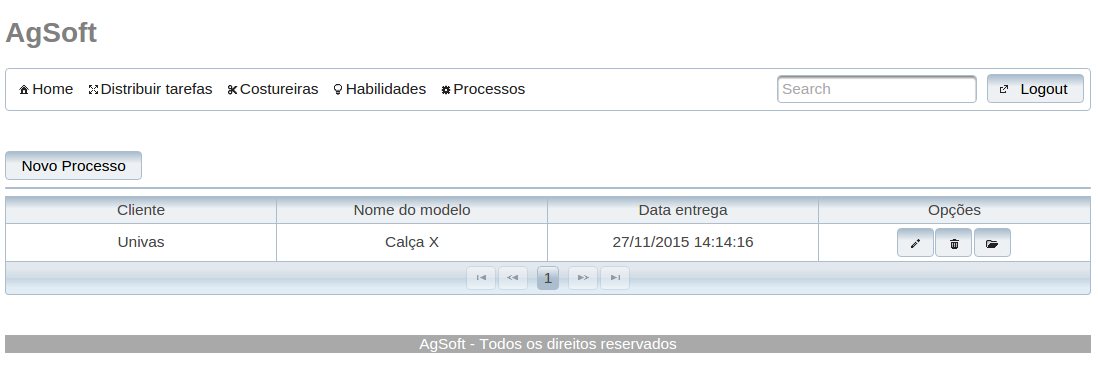
\includegraphics[scale=0.4]{./imagens/teste_processo.png}}
	\caption[Criação de um processo]
	{Criação de um processo \textbf{Fonte:} Desenvolvido pelos autores}
	\label{fig:exemplo1}
\end{figure}

\par Todo processo ao ser criado, por padrão já contém as atividades principais
que são o carimbo e a finalização conforme mostra a Figura
~\ref{fig:processo_cadastrado}:

\begin{figure}[h!]
	\centerline{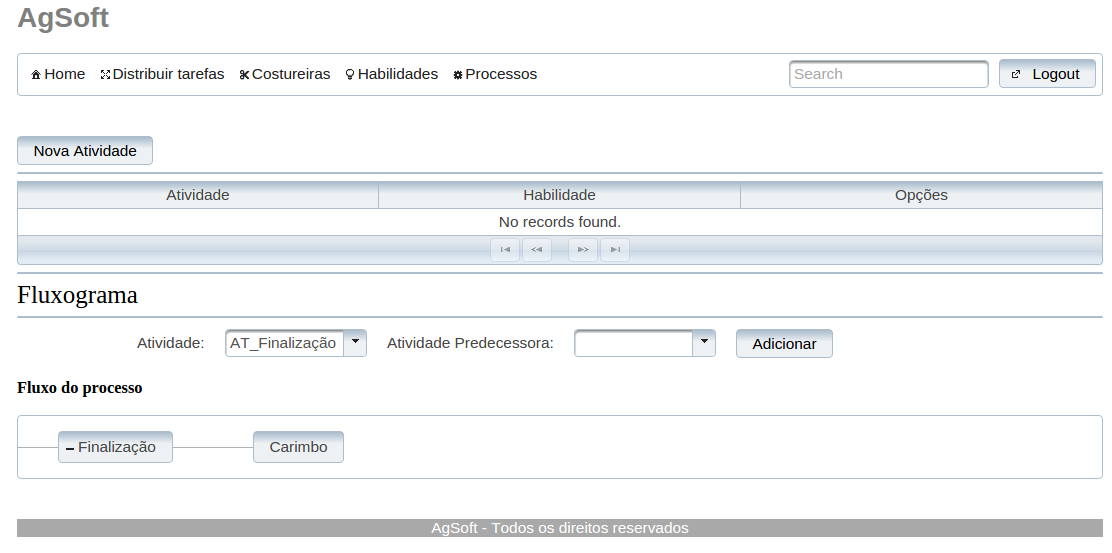
\includegraphics[scale=0.4]{./imagens/tela_processo_teste1.png}}
	\caption[Detalhes do processo cadastrado]
	{Detalhes do processo cadastrado \textbf{Fonte:} Desenvolvido pelos autores}
	\label{fig:processo_cadastrado}
\end{figure}

\par Após a criação do processo é preciso definir quais costureiras possuem a
habilidade para realizar as atividades que compõe o processo. Vale ressaltar que
a atividade Carimbo é realizada somente pelo proprietário da fábrica pois é a
atividade onde serão distribuídas as peças para serem produzidas e por isso
também esta atividade esta como atividade principal.

\par Será definido para realizar a atividade Finalização as costureiras
Maria e Duda, ambas cobram o mesmo valor por peça porém o tempo
gasto em que cada uma gasta para fabricar a peça é diferente conforme mostra
a Figura ~\ref{fig:costureira_habilidade}:

\newpage

\begin{figure}[h!]
	\centerline{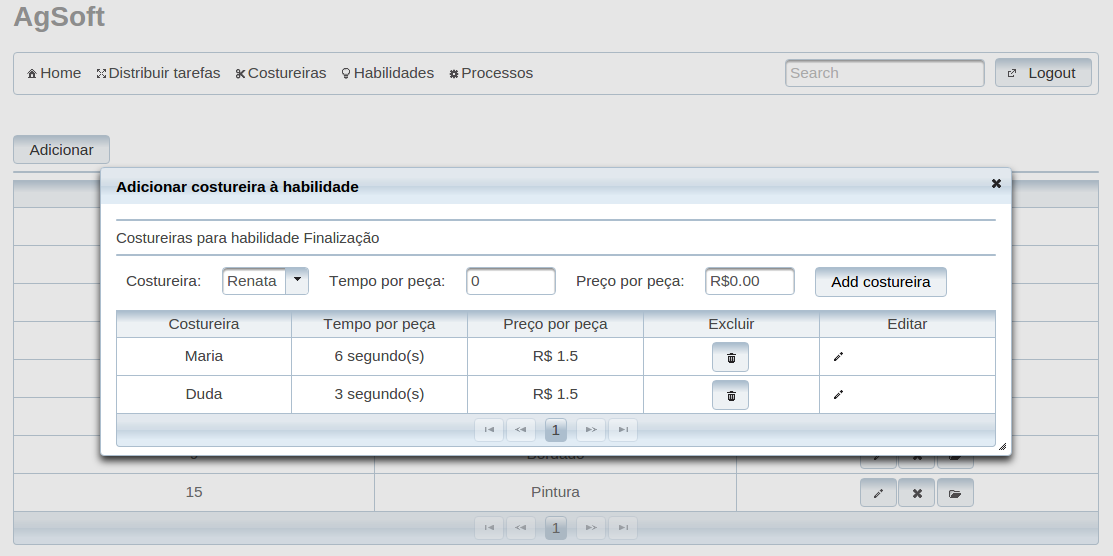
\includegraphics[scale=0.4]{./imagens/tela_habilidade_teste1.png}}
	\caption[Demonstração inserir costureira à habilidade]
	{Demonstração inserir costureira à habilidade \textbf{Fonte:} Desenvolvido pelos autores}
	\label{fig:costureira_habilidade}
\end{figure}


\par Feito isso, pode-se iniciar o processo de distribuição
das atividades, através do menu Distribuição de Tarefas.
Ao acessar a página todos os processos criados serão
listados como mostra a Figura ~\ref{fig:distribuicao_tarefas}:

\begin{figure}[h!]
	\centerline{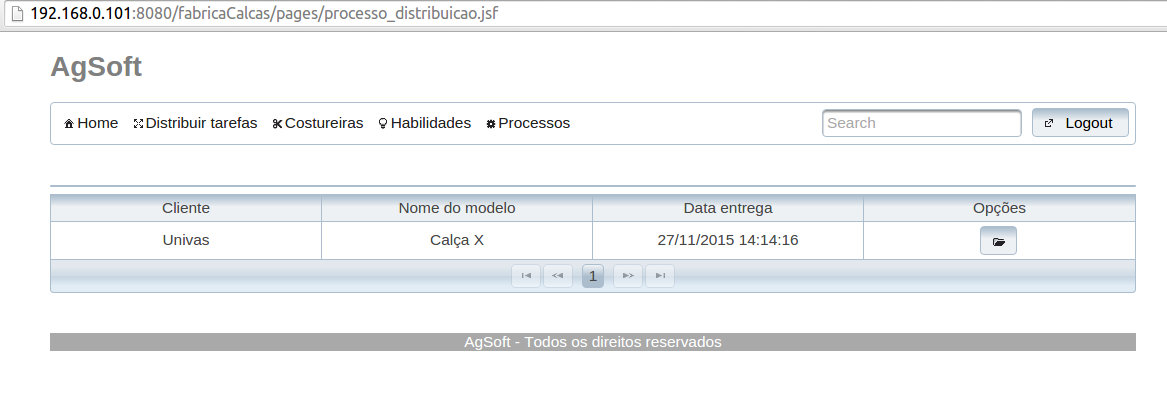
\includegraphics[scale=0.4]{./imagens/tela_distribuicao_tarefas.png}}
	\caption[Demonstração tela de dritribuição de tarefas]
	{Demonstração tela de dritribuição de tarefas \textbf{Fonte:} Desenvolvido pelos autores}
	\label{fig:distribuicao_tarefas}
\end{figure}


\par Ao clicar no botão abrir será mostrado a tela para que o usuário insira os
dados como número de peças, total de peças por lote e data inicio. Depois de
inseridos os dados a ao clicar no botão Iniciar distribuição o sistema executa
toda a parte de algoritmos genéticos e retorna para o usuário a melhor solução
encontrada com base nos dados inseridos conforme mostra a Figura
~\ref{fig:resultado_distribuicao_teste1}:


\begin{figure}[h!]
	\centerline{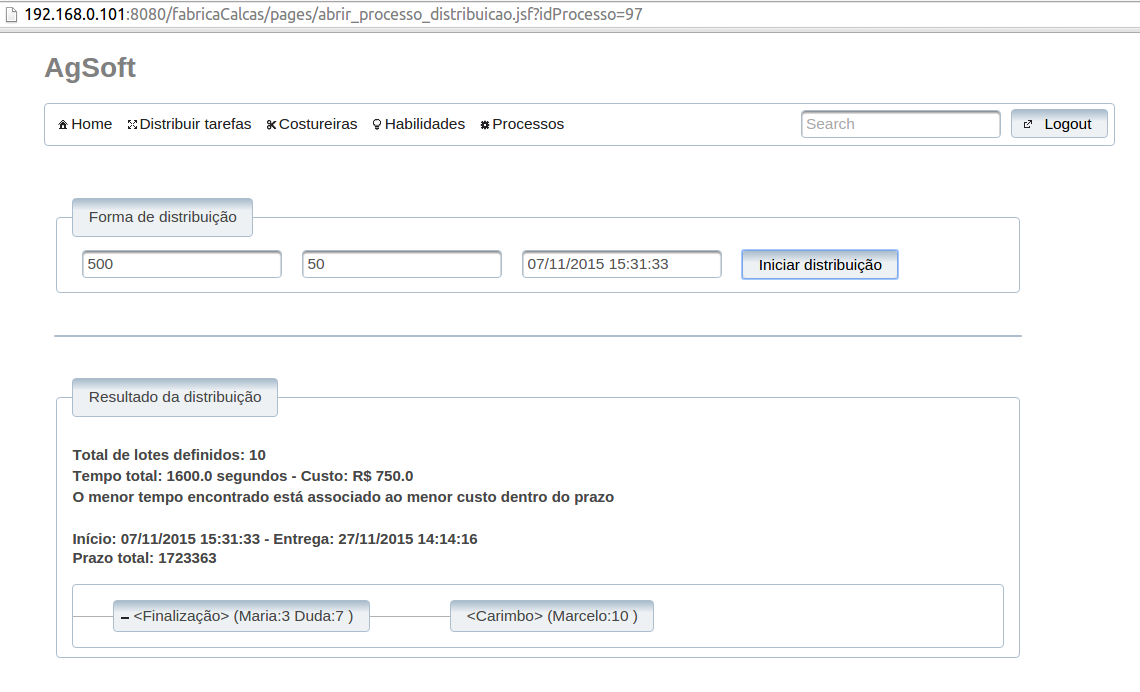
\includegraphics[scale=0.4]{./imagens/resultado_distribuicao_teste1.png}}
	\caption[Resultado da distribuição de lotes]
	{Resultado da distribuição de lotes \textbf{Fonte:} Desenvolvido pelos autores}
	\label{fig:resultado_distribuicao_teste1}
\end{figure}

\par Conforme ilustrado na Figura ~\ref{fig:costureira_habilidade}, Maria possui
o tempo de produção maior que Duda, por isso ela recebe um número menor de lotes
para produzir conforme ilustrado na Figura
~\ref{fig:resultado_distribuicao_teste1}

\par Se o tempo de cada costureira for alterado, um novo resultado será
retornado levando em consideração as alterações. Para isto, será definido para
Maria o tempo de 4 segundos e para Duda o tempo de 7 segundos conforme ilustra a
Figura ~\ref{fig:tempo_costureiras}: 

\newpage

\begin{figure}[h!]
	\centerline{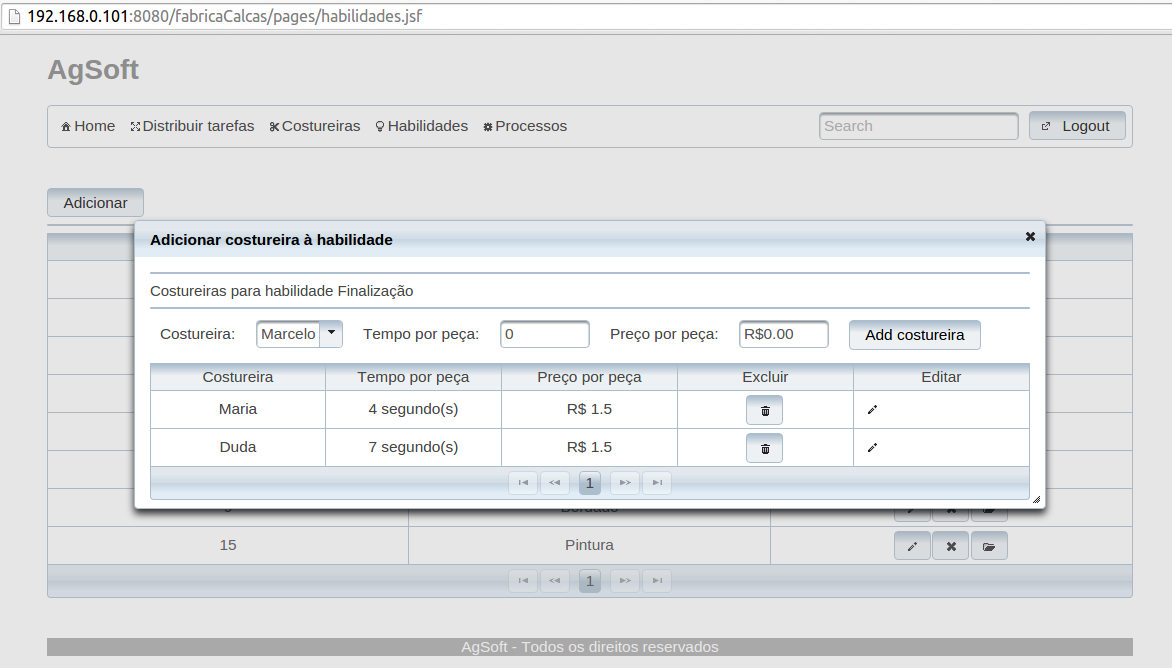
\includegraphics[scale=0.4]{./imagens/alterando_tempo_costureira.png}}
	\caption[Tempo de produção entre as costureiras]
	{Tempo de produção entre as costureiras \textbf{Fonte:} Desenvolvido pelos autores}
	\label{fig:tempo_costureiras}
\end{figure}



\par Após executar novamente a distribuição será retornado um novo resultado
ilustrado na Figura ~\ref{fig:novo_resultado_distribuicao_teste1}:



\begin{figure}[h!]
	\centerline{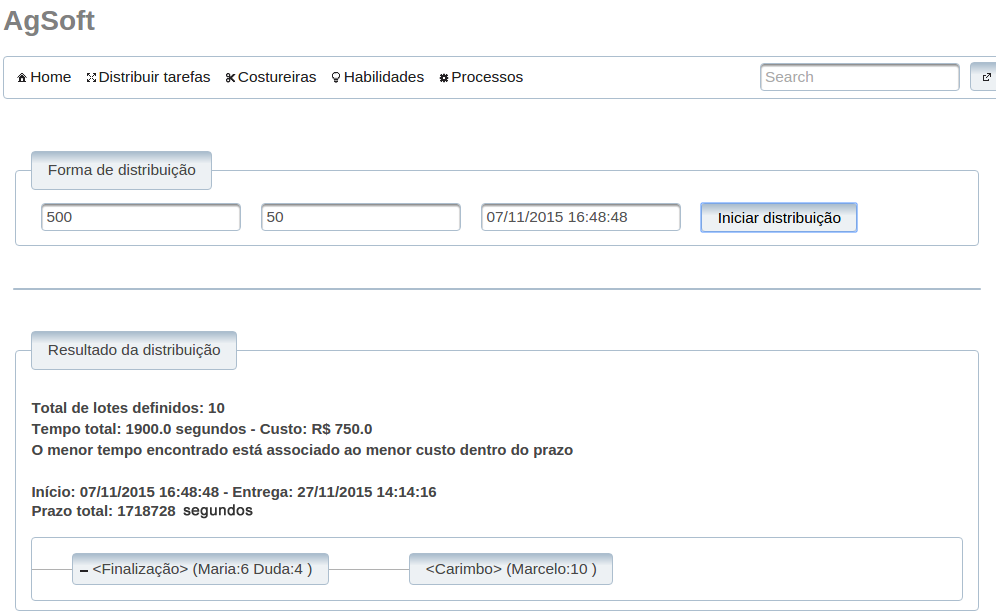
\includegraphics[scale=0.4]{./imagens/novo_resultado_alterado_tempo_teste1.png}}
	\caption[Resultado da distribuição de lotes]
	{Resultado da distribuição de lotes \textbf{Fonte:} Desenvolvido pelos autores}
	\label{fig:novo_resultado_distribuicao_teste1}
\end{figure}

\par Neste resultado Maria obtém mais lotes que Duda para produzir pois o seu
tempo de produção é menor. O algoritmo foi configurado para ter 1000
gerações e 80 indivíduos em cada população, além disso a taxa de indivíduos estrangeiros e de mutação 
foram de 0,5\% e 0,05\% respectivamente.


\section{Teste considerando o custo de produção}

\par Este teste segue o mesmo procedimento do teste realizado na seção 4.1,
porém o tempo de produção entre as costureiras será o mesmo e o custo será
alterado.

\par O processo assim como o processo da seção 4.1 irá conter as atividades
Carimbo e Finalização. 
Será definido o tempo de 5 segundos para as costureiras Maria e Duda e o preço por 
peça R\textdollar 1,50 e R\textdollar
2,70 respectivamente. Além disso foi definido os mesmos valores X e Y  
relativos a posição geografica para Maria e Duda, de forma a manter o tempo de
transporte semelhantes para ambas. A Figura
~\ref{fig:custo_entre_costureiras} mostra a definição de tempo e custo para
ambas as costureiras:



\begin{figure}[h!]
	\centerline{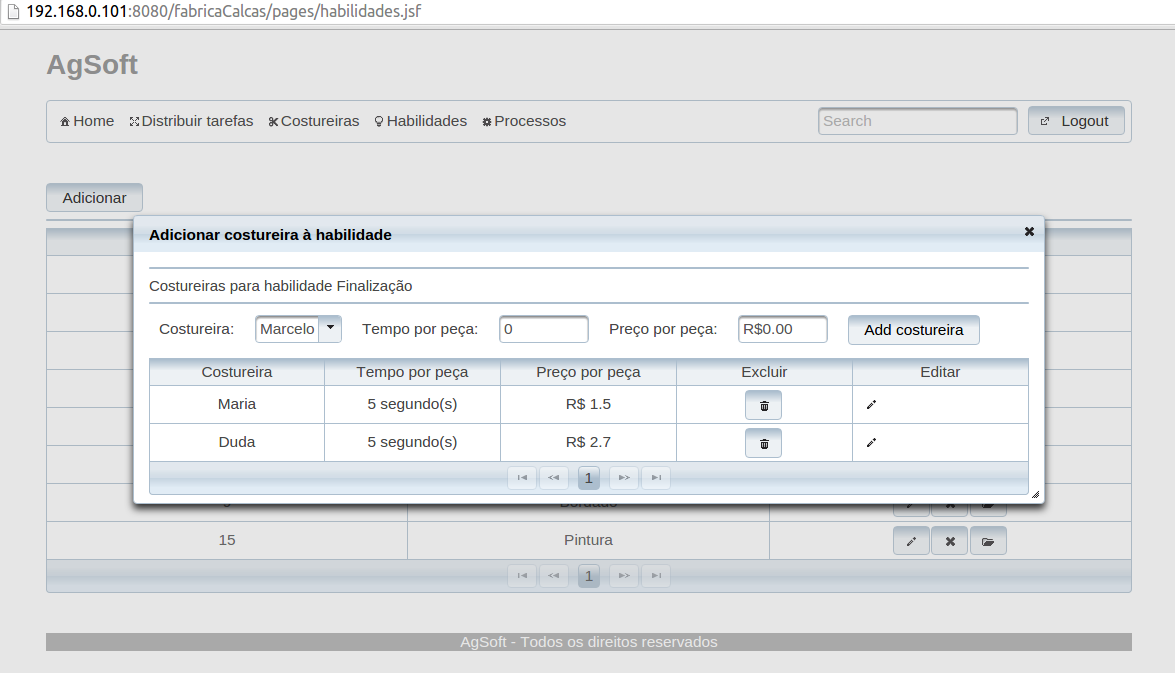
\includegraphics[scale=0.4]{./imagens/custo_entre_costureiras_teste2.png}}
	\caption[Custo entre as costureiras atividade Finalização]
	{Custo entre as costureiras atividade Finalização \textbf{Fonte:} Desenvolvido pelos autores}
	\label{fig:custo_entre_costureiras}
\end{figure}



\par Ao executar a aplicação é retornado a seguinte distribuição ilustrada na
Figura ~\ref{fig:resultado_custo}:

\newpage

\begin{figure}[h!]
	\centerline{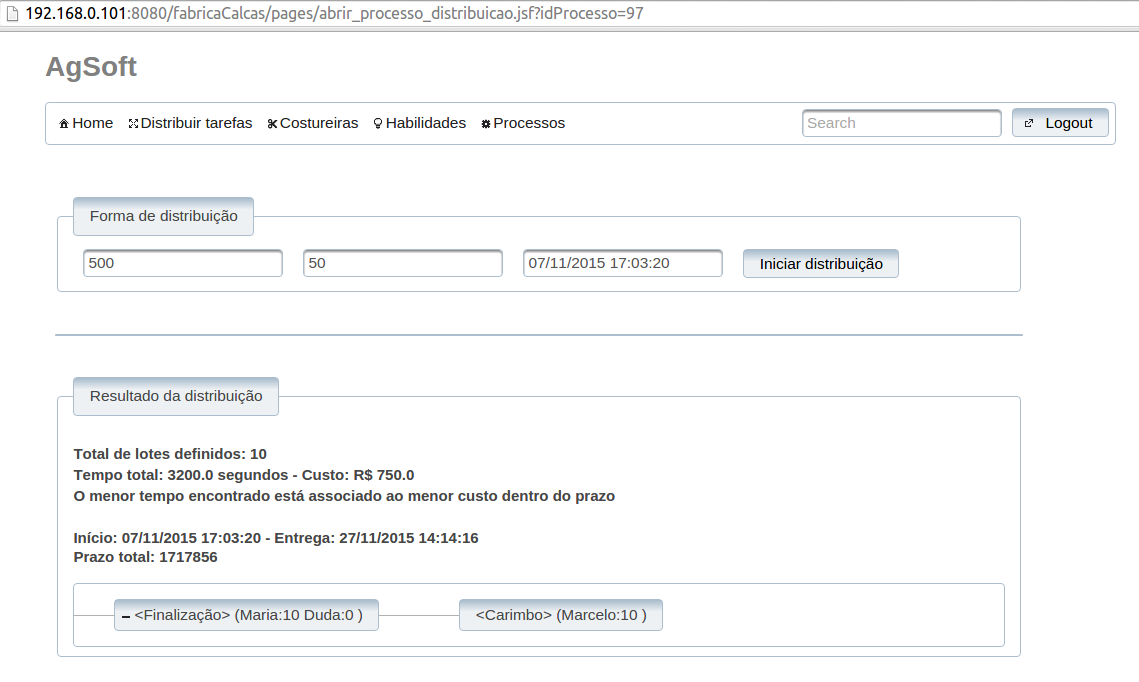
\includegraphics[scale=0.4]{./imagens/resultado_teste2.png}}
	\caption[Custo entre as costureiras atividade Finalização]
	{Custo entre as costureiras atividade Finalização \textbf{Fonte:} Desenvolvido pelos autores}
	\label{fig:resultado_custo}
\end{figure}

\par Com base no resultado obtido, o algoritmo interpretou que pelo fato de
Maria e Duda obter o mesmo tempo de produção e Duda ter um preço por peça
bem superior que o de Maria, Duda não recebeu nenhum lote para produzir, pois neste
caso é possível que Maria produza sozinha os lotes dentro do prazo de entrega do
processo. Caso Maria não conseguisse produzir os lotes no prazo estipulado, o
algoritmo adequa a distribuição distribuindo alguns lotes para Duda para
conseguir alcançar o prazo de entrega, toda via, fazendo isto, o custo tende a
almentar, este caso será mostrado com mais detalhes na seção 4.3.

\par Caso Maria e Duda obtvessem o mesmo tempo, o mesmo preço e a mesma posição
X e Y o algoritmo distribui lotes para Duda pois, mesmo a costureira Maria
conseguindo fabricar as peças dentro do prazo, se Duda receber alguns lotes para produzir
isto não interferirá no preço final como mostra a Figura
~\ref{fig:resultado_tudo_igual}.
\newpage

\begin{figure}[h!]
	\centerline{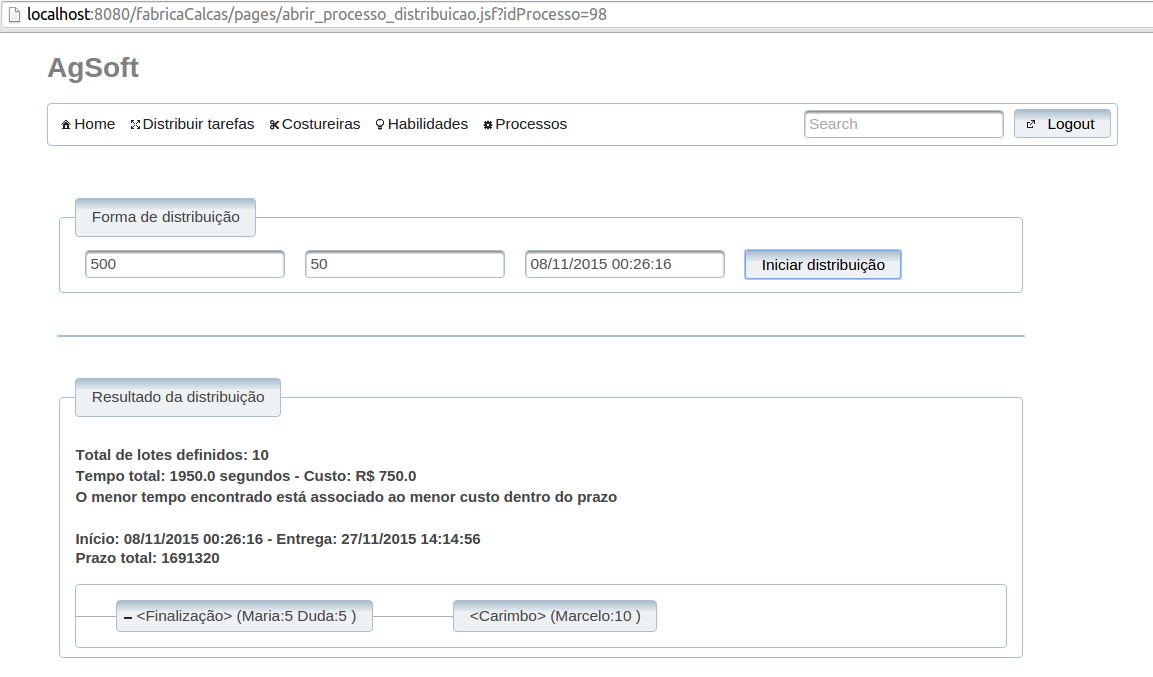
\includegraphics[scale=0.4]{./imagens/resultado_tudo_igual_teste2.png}}
	\caption[Custo entre as costureiras atividade Finalização]
	{Custo entre as costureiras atividade Finalização \textbf{Fonte:} Desenvolvido pelos autores}
	\label{fig:resultado_tudo_igual}
\end{figure}

\section{Teste tempo x custo e prazo de entrega}

\par Este teste foi realizado para demonstrar como fica o tempo de
produção e o custo quando o prazo de entrega é curto,
assim mesmo que uma costureira for inviável pelo tempo ou custo, ela poderá
receber ou não lotes para produzir para que seja cumprido o prazo de entrega.

\par Para isto as costureiras que possuem a habilidade Finalização ficarão com
as seguintes configurações como ilustra a Figura
~\ref{fig:configuracao_habilidade_costureira_teste3}

\newpage

\begin{figure}[h!]
	\centerline{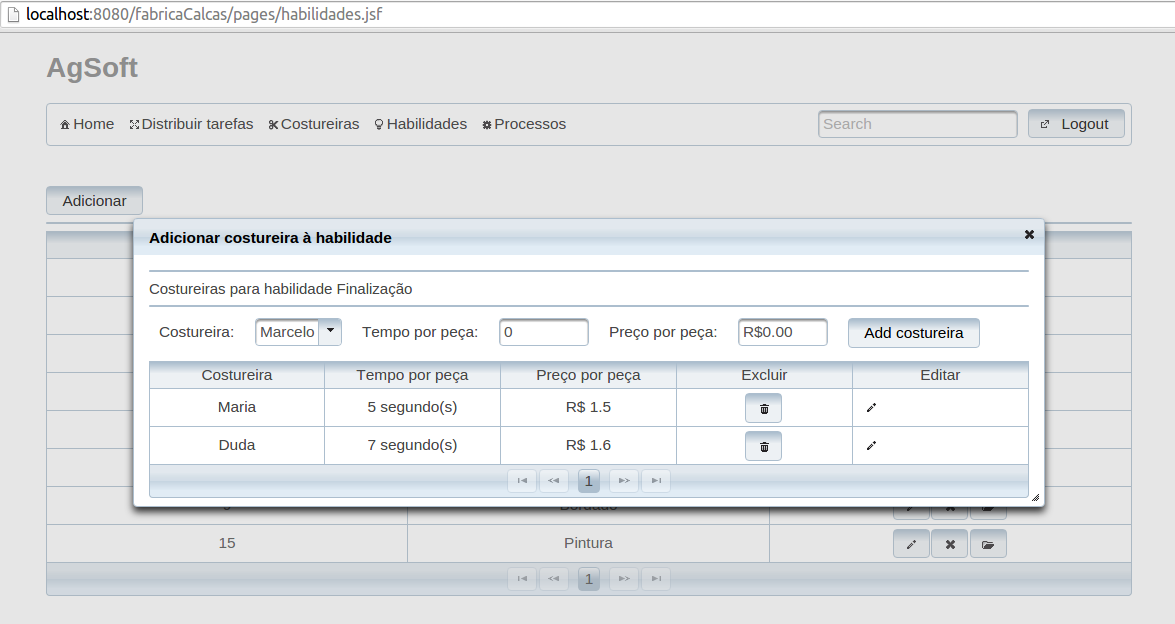
\includegraphics[scale=0.4]{./imagens/cofiguracao_habilidade_teste3.png}}
	\caption[Custo entre as costureiras atividade Finalização]
	{Custo entre as costureiras atividade Finalização \textbf{Fonte:} Desenvolvido pelos autores}
	\label{fig:configuracao_habilidade_costureira_teste3}
\end{figure}


\par A Figura ~\ref{fig:resultado1_teste3} mostra o resultado
com base nas configurações da habilidade Finalização mostrada na Figura
~\ref{fig:configuracao_habilidade_costureira_teste3}.

\begin{figure}[h!]
	\centerline{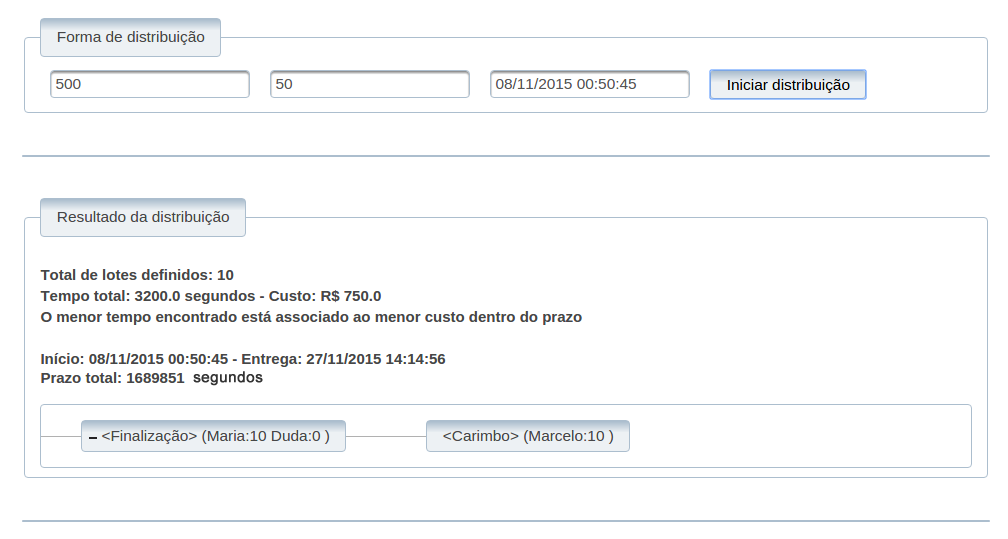
\includegraphics[scale=0.4]{./imagens/resultado1_teste3.png}}
	\caption[Custo entre as costureiras atividade Finalização]
	{Custo entre as costureiras atividade Finalização \textbf{Fonte:} Desenvolvido pelos autores}
	\label{fig:resultado1_teste3}
\end{figure}

\par Como ilustrado na Figura ~\ref{fig:resultado1_teste3} a costureira Duda não
recebe nenhum lote pois possui um tempo de produção e custo maior que Maria,
porém se caso o prazo de entrega for menor, Duda poderá dependendo do prazo,
receber lotes para produzir mesmo que o tempo e o custo finais aumentem para
atender o prazo de entrega.

A Figura ~\ref{fig:resultado2_teste3} mostra a distribuição de lotes entre as
costureiras com alteração na data de inicio do processo.

\begin{figure}[h!]
	\centerline{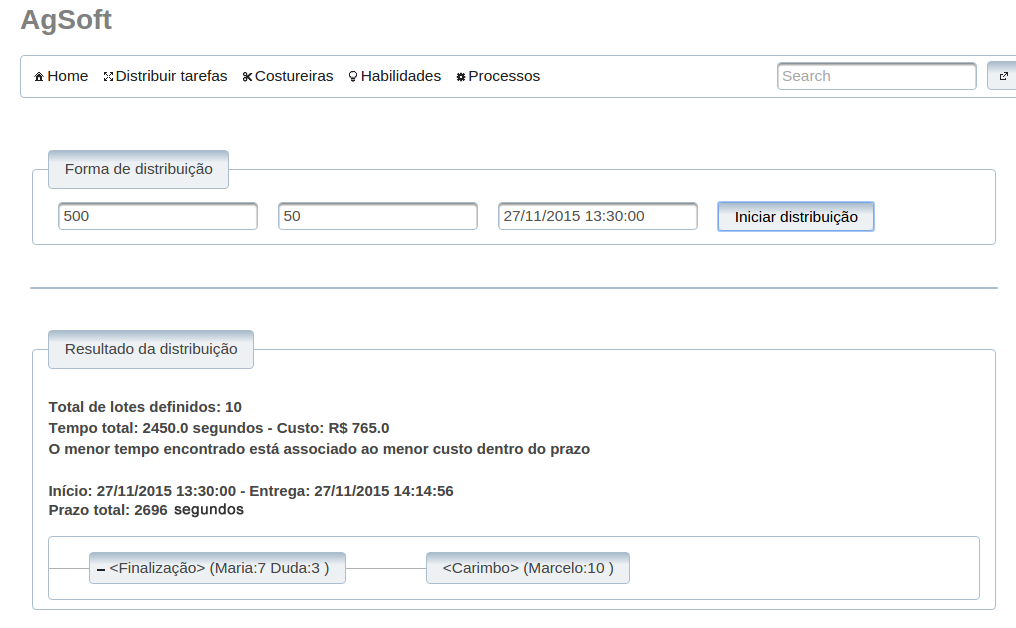
\includegraphics[scale=0.4]{./imagens/resultado2_teste3.png}}
	\caption[Custo entre as costureiras atividade Finalização]
	{Custo entre as costureiras atividade Finalização \textbf{Fonte:} Desenvolvido pelos autores}
	\label{fig:resultado2_teste3}
\end{figure}

\par Como ilustrado na Figura ~\ref{fig:resultado2_teste3} a costureira Duda
recebe 3 lotes para produzir, assim, o tempo de produção e custo aumentam com
relação ao resultado da Figura ~\ref{fig:resultado1_teste3}, porém o prazo de
entrega é cumprido.


\section{Teste considerando o tempo de transporte}

\par Este teste foi realizado para demonstrar que mesmo as costureiras possuindo
o tempo e custo iguais, a distancia entre a fábrica pode determinar a
distribuição dos lotes.


\par Para isto foi necessário cadastrar um valor X e Y para cada costureira que
representa sua localização conforme mostra a Figura ~\ref{fig:add_xy_costureira_teste4}.

\newpage

\begin{figure}[h!]
	\centerline{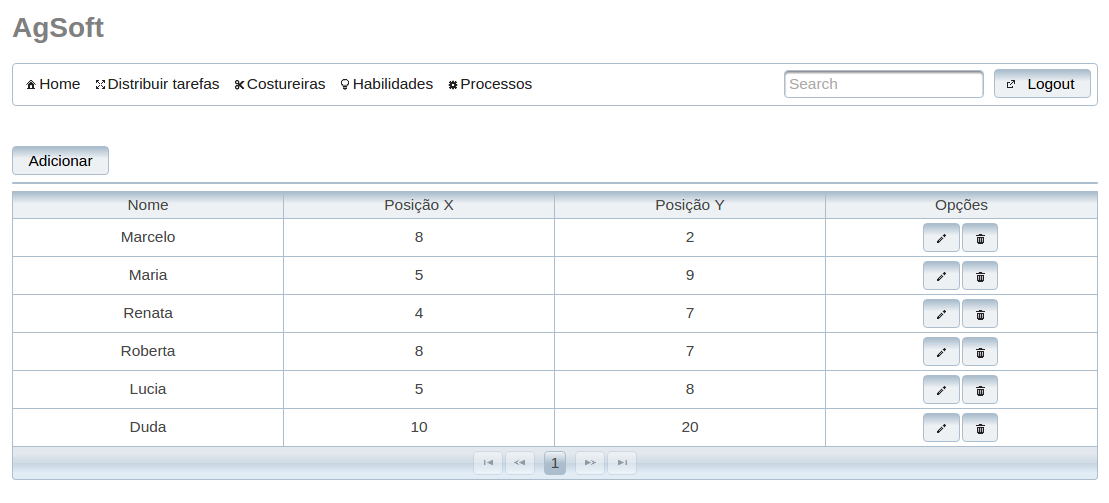
\includegraphics[scale=0.3]{./imagens/posicao_xy_costureiras_teste4.png}}
	\caption[Caso de teste com tempo de distribuição]
	{Caso de teste com tempo de distribuição \textbf{Fonte:} Desenvolvido pelos autores}
	\label{fig:add_xy_costureira_teste4}
\end{figure}



\par Neste teste foi considerado apenas o tempo de transporte, logo o tempo de
confecção por peça das costureiras da atividade Finalização possuem o mesmo
valor de tempo e custo, conforme mostra a Figura
~\ref{fig:at_finalizacao_teste4}.


\begin{figure}[h!]
	\centerline{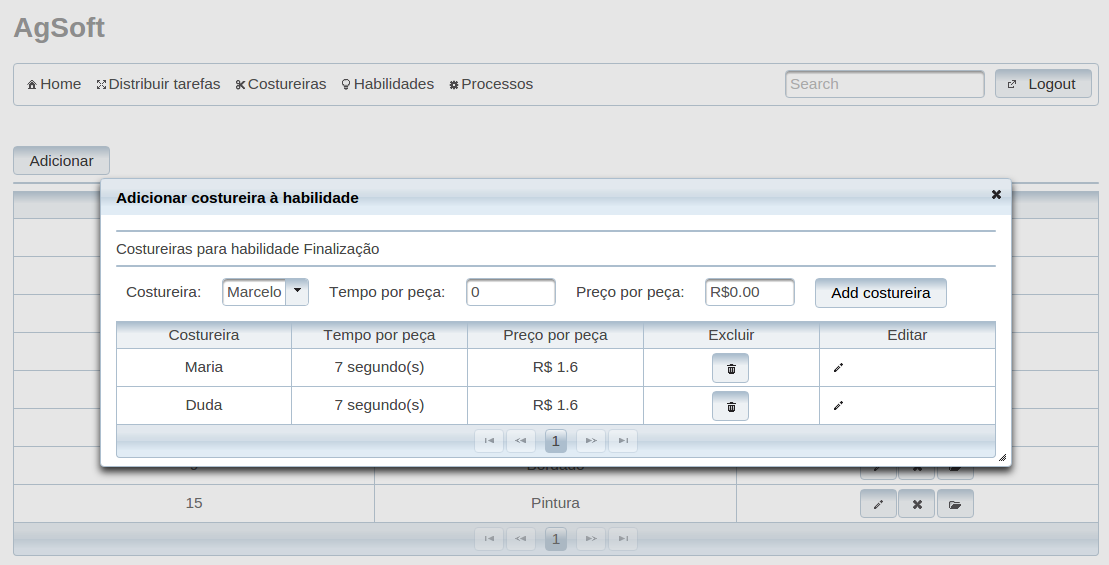
\includegraphics[scale=0.3]{./imagens/cofig_at_finalizaca_teste4.png}}
	\caption[Caso de teste com tempo de distribuição]
	{Caso de teste com tempo de distribuição \textbf{Fonte:} Desenvolvido pelos autores}
	\label{fig:at_finalizacao_teste4}
\end{figure}

\newpage

\par Feito isso foi iniciado então o processo de distribuição das atividades,
através do menu Distribuição de Tarefas, a Figura
~\ref{fig:resultado_transporte_teste4} mostra o resultado obtido.


\begin{figure}[h!]
	\centerline{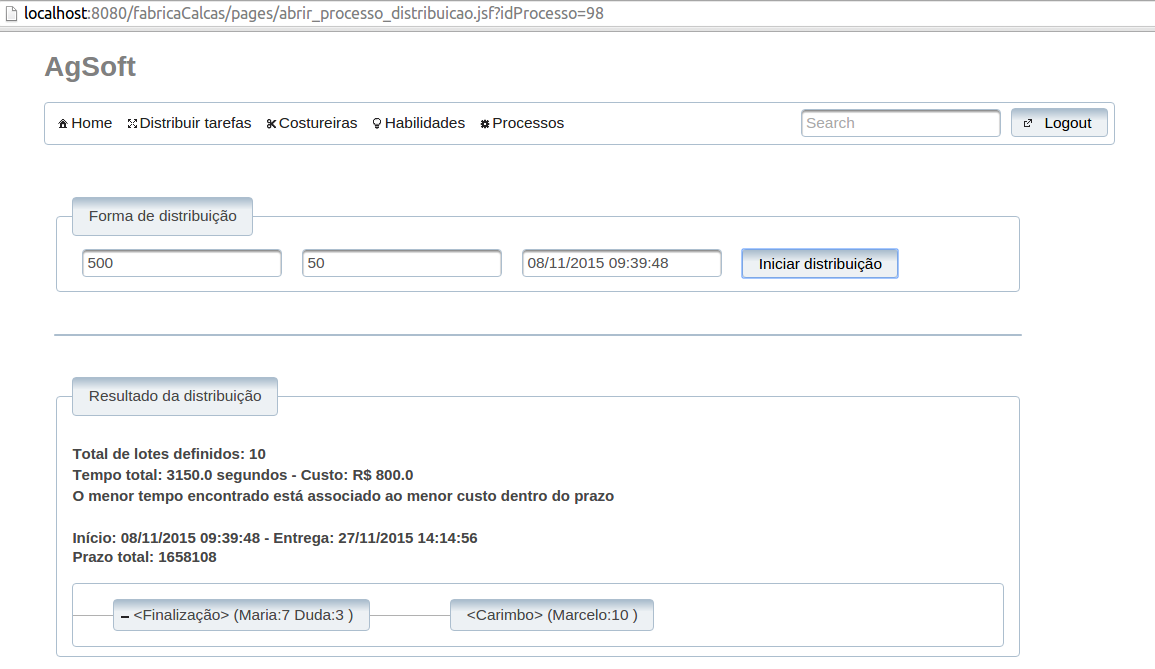
\includegraphics[scale=0.3]{./imagens/resultado_transporte_teste4.png}}
	\caption[Distribuição das atividades]
	{Distribuição das atividades \textbf{Fonte:} Desenvolvido pelos autores}
	\label{fig:resultado_transporte_teste4}
\end{figure}

\par Como mostrado na figura ~\ref{fig:add_xy_costureira_teste4}, a costureira
Duda fica mais distante da fábrica por isso recebe menos lotes para produzir em
relação a costureira Maria.

\section{Teste adicionando mais atividades}

\par Neste caso deve-se considerar o tempo de transporte entre as costureiras da atividade Frente e a fábrica 
para a retirada dos materiais e o tempo entre tais costureiras e a costureira
responsável pela Finalização, para isso foi adicionado no processo a atividade
frente conforme mostra a Figura ~\ref{fig:add_frente_teste4}.


\begin{figure}[h!]
	\centerline{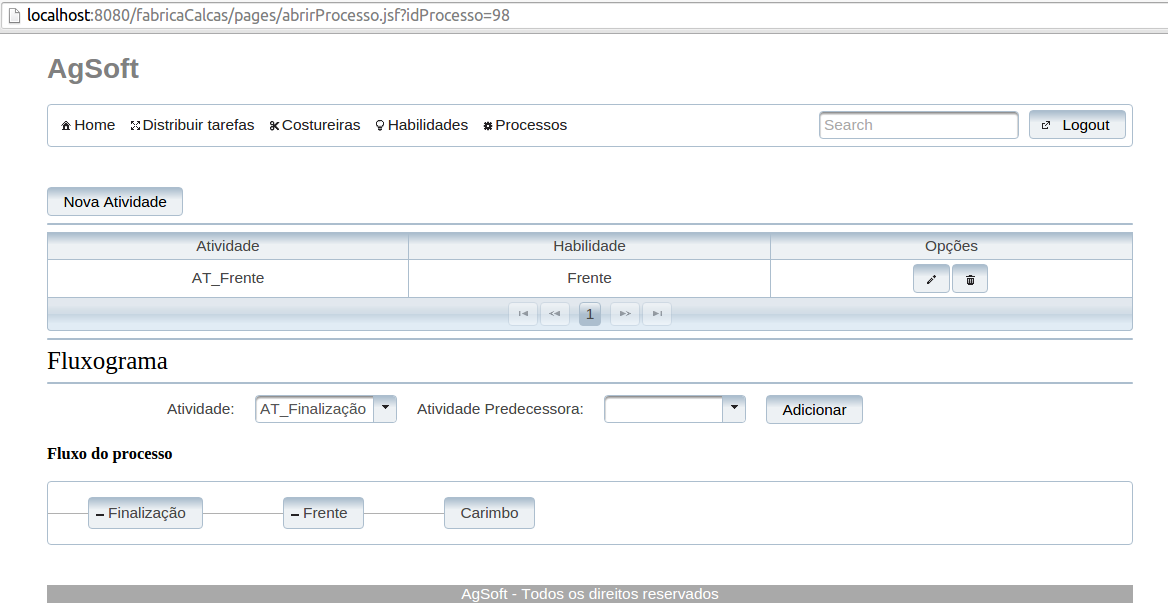
\includegraphics[scale=0.3]{./imagens/adicionar_atividade_frente_teste4.png}}
	\caption[Caso de teste com tempo de distribuição]
	{Caso de teste com tempo de distribuição \textbf{Fonte:} Desenvolvido pelos autores}
	\label{fig:add_frente_teste4}
\end{figure}


\par Foi adicionado na habilidade frente a costureira Roberta para que esta
possa realizar a atividade frente do processo.
\par A Figura mostra a costureira adicionada na habilidade frente.

\begin{figure}[h!]
	\centerline{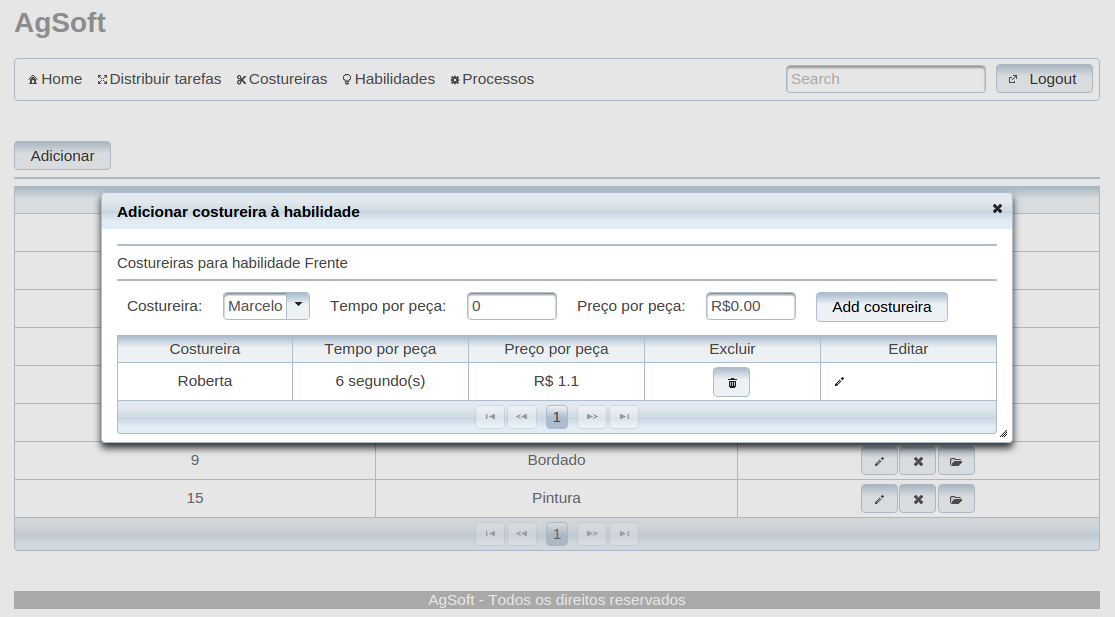
\includegraphics[scale=0.3]{./imagens/costureira_frente_teste4.png}}
	\caption[Caso de teste com tempo de distribuição]
	{Caso de teste com tempo de distribuição \textbf{Fonte:} Desenvolvido pelos autores}
	\label{fig:add_costureira_frente_teste4}
\end{figure}



%%%%%%%%%%%%%%%%%%%%%%%%%%%%%%%%%%%%%%%%%%%%%%%%%%%%%%%%%%%%%%%

\par Após clicar no botão "Iniciar Distribuição", o algoritmo distribuiu os lotes para as costureiras das atividades
 finalização e frente o qual o tempo total encontrado foi de 1700 segundos,
 conforme mostra a Figura 34. Neste caso o algoritmo distribuiu 5 peças para cada costureira da parte da frente, logo, como a atividade de finalização possui somente uma costureira,
 a Roberta e a Tereza irão passar 5 peças cada uma para a Josi, que faz a
 finalização. Conforme descrito no quadro metodológico, o cálculo da distância entre as costureiras é realizado através da fórmula euclidiana multiplicando-se o resultado por 100.
 A Figura 35 mostra as distâncias entre as costureiras calculadas através desta
 fórmula com suas posições X e Y.
  
  \newpage
  
  \begin{figure}[h!]
  	\centerline{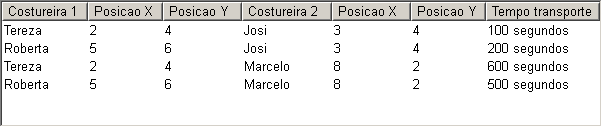
\includegraphics[scale=0.7]{./imagens/test_case_2_tempo_distribuicao.png}}
  	\caption[Distribuição do tempo]
  	{Distribuição do tempo  \textbf{Fonte:} Desenvolvido pelos autores}
  	\label{fig:exemplo1}
  \end{figure}
 
\par Considerando que as costureiras Roberta e Tereza gastam o mesmo tempo para fazer a frente e que o tempo de transporte 
entre a Tereza e a Josi é menor (100 a menos que entre a Roberta e a Josi), o algoritmo deveria distribuir mais peças a Tereza,
porém os materiais devem ser pegos na casa do Marcelo e, neste caso, o tempo de transporte entre a Tereza e o Marcelo é 100 
a mais que o tempo de transporte entre a Roberta e o Marcelo, logo o algoritmo entendeu que o tempo se igualou e definiu
o mesmo número de peças para cada costureira.

\par Existem outros resultados a serem documentados incluindo a questão de custo, porém até a entrega da discussão dos resultados
os mesmos não estavam elaborados.
